\chapter{Overall Concept of the Developed Solution}
\label{cha:concept}

In this chapter, the first research question is answered by presenting an extension
of the UME (Unified Microservice Engineering) approach with a monitoring concept.
First, the UME approach is described in detail in Section \ref{sec:ume_approach}.
This is followed by an explanation of where monitoring fits into the DevOps concept
in Section \ref{sec:devops_pattern_feedback}.
Finally, the developed monitoring concept for the UME approach is presented
in Section \ref{sec:integration_monitoring_ume}.

\section{The Unified Microservice Engineering Approach}
\label{sec:ume_approach}

\begin{figure}[tb]
	\centering
	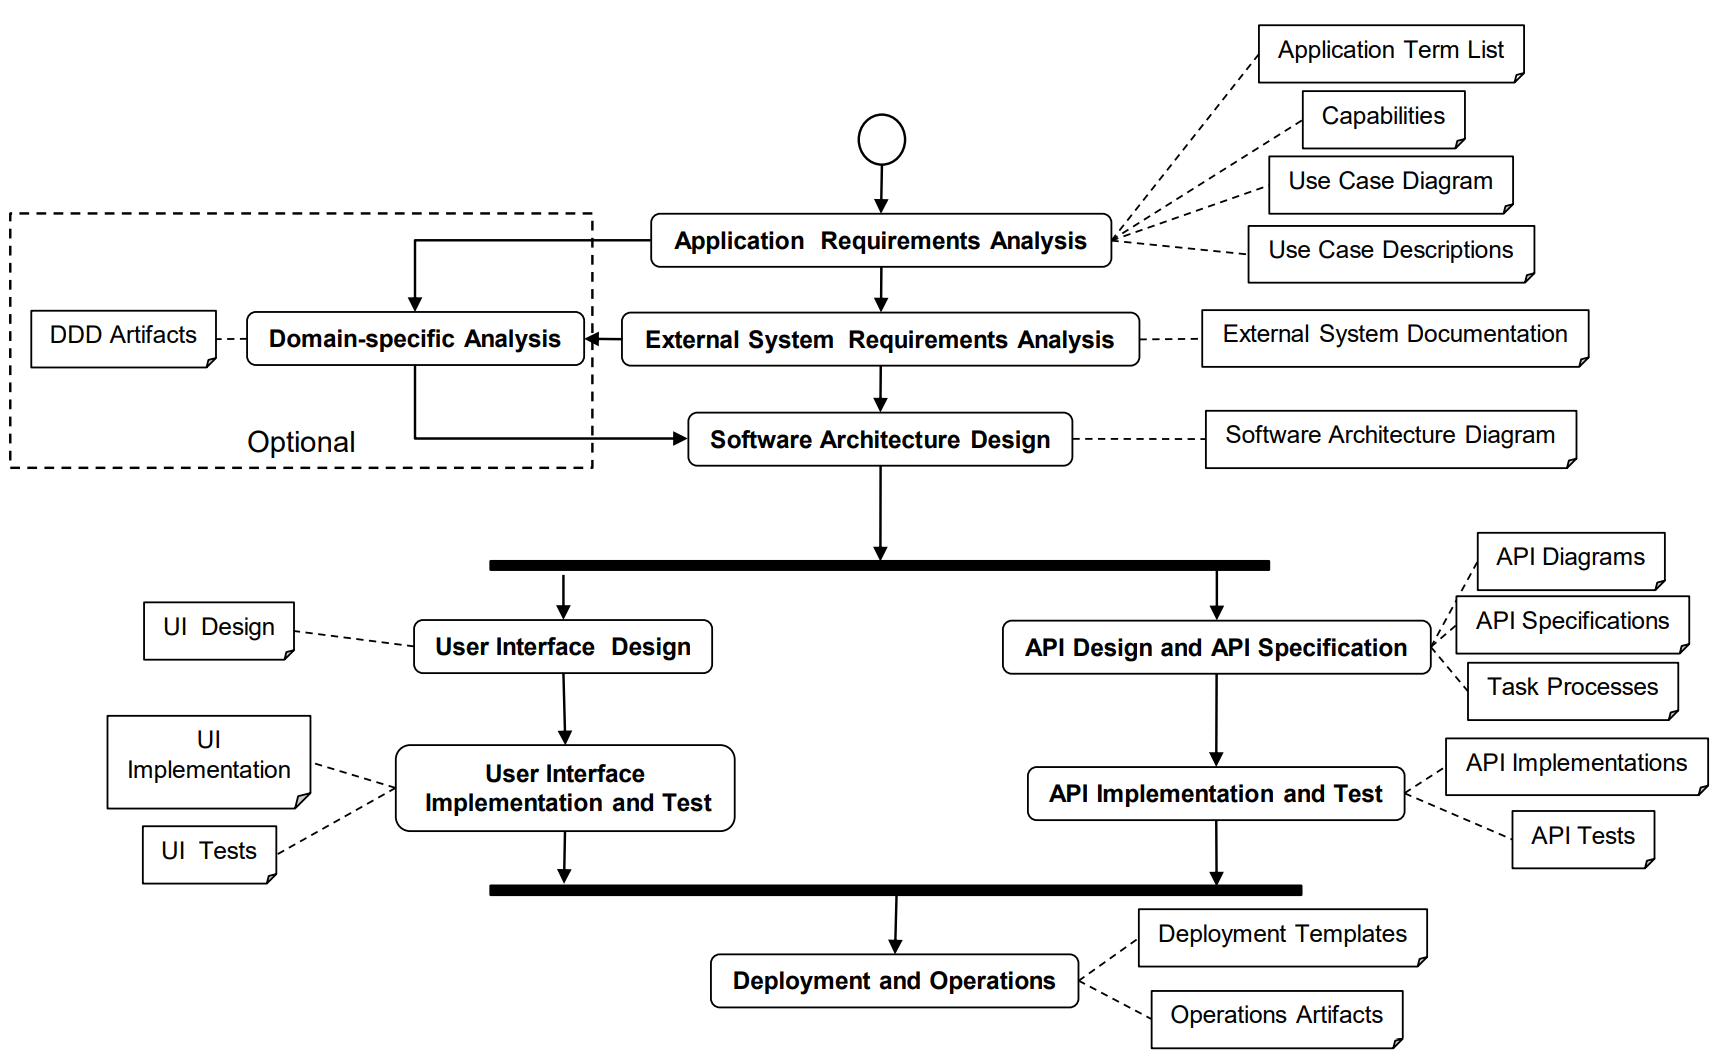
\includegraphics[width=\textwidth]{figures/4.1_ume_approach.png}
	\caption{Unified Microservice Engineering Approach \cite{CM-W-OVW}}
	\label{fig:ume_approach}
\end{figure}

The UME (Unified Microservice Engineering) approach is a software development
process by the C\&M (Cooperation \& Management) research group
for the development of microservice-based applications.
An overview of the whole approach can be seen in Figure \ref{fig:ume_approach}.
The UME approach consists of four phases: analysis, design, implementation and test,
and deployment and operation. The approach can optionally be extended with domain-driven aspects.
The analysis phase starts with the application requirements analysis
which analyzes and describes the requirements of the application that is to be developed.
This consists of creating an application term list that specifies the meaning
of application-related terms for all involved parties. The application term list
is not a part of the ubiquitous language as it is used in domain-driven design (DDD) because it
may span multiple different domains. Contrary, the ubiquitous language of DDD is always
specific to a single domain. Using the terms from the application term list,
capabilities and use cases are defined for the application. 
For each capability, a separate use case diagram is created.
The use cases from each use case diagram are further specified in use case descriptions.
Optionally, the application requirements analysis may be extended with additional artifacts
like a business vision and goals or an application sketch.
The standard analysis phase of the UME approach is concluded with the external system requirements analysis.
This analysis focuses on specifying the requirements for external systems which will be used
by the application. Examples of such external systems are databases, enterprise applications,
and business services. The results of this analysis are documented in the external system documentation.
In the case that the UME approach is extended with domain-driven aspects,
the analysis phase consists of an additional step: the domain-specific analysis.
This step encapsulates the standard DDD and its artifacts like ubiquitous languages
and domain models.

\begin{figure}[tb]
	\centering
	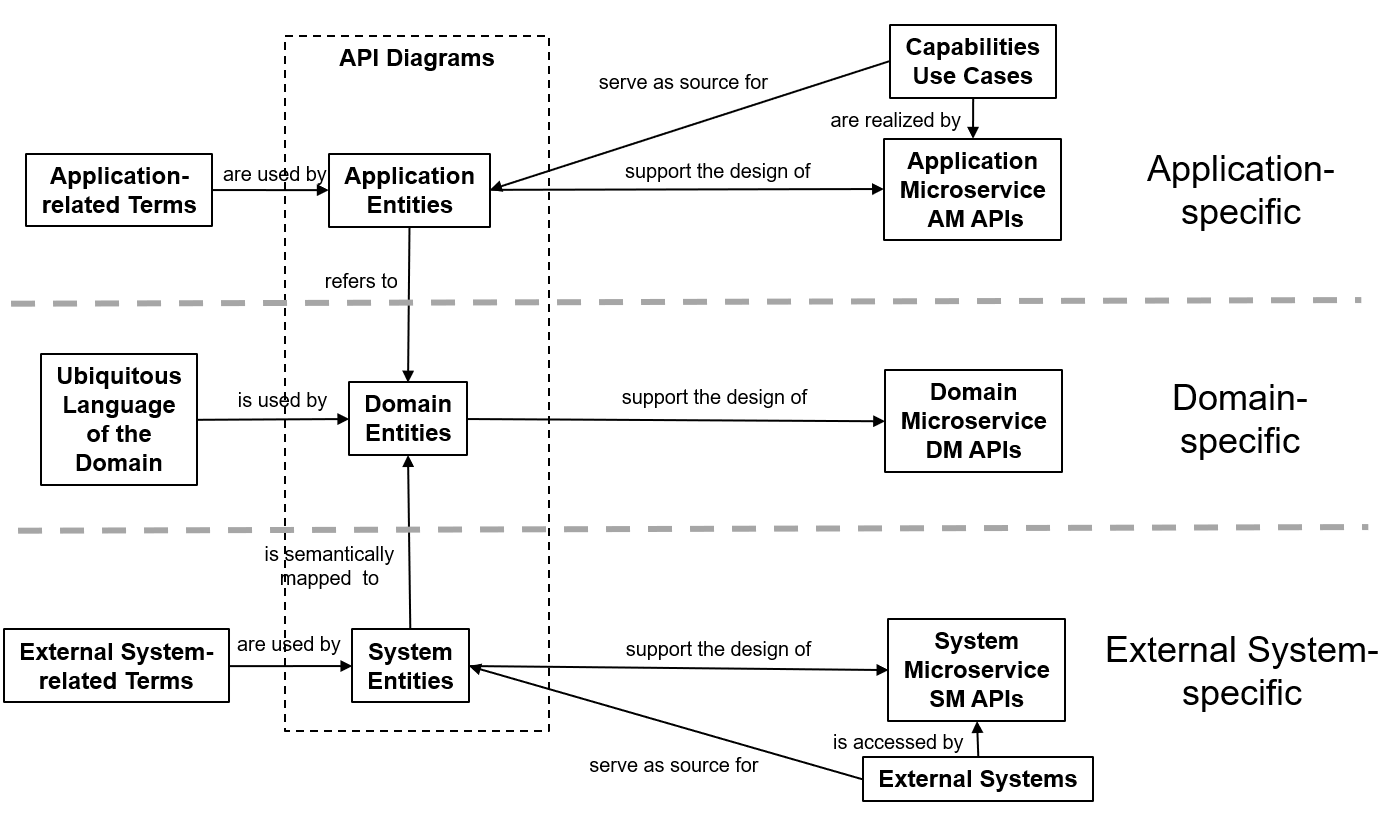
\includegraphics[width=\textwidth]{figures/4.2_ume_approach_api_design.png}
	\caption{UME Approach - API Design \cite{CM-W-DES}}
	\label{fig:ume_approach_api_design}
\end{figure}

After the analysis phase comes the design phase which starts with the software architecture design.
The software architecture of the application consists of application, domain, and system APIs.
An overview of these APIs, their entities and different analysis artifacts can be seen in Figure \ref{fig:ume_approach_api_design}.
The application APIs are derived from use cases and directly provide the functionality set forth
by the use cases. There is a one-to-one mapping between the methods of the application APIs and the use cases.
The domain APIs provide domain-specific logic as a layer of abstraction
on top of the system APIs.
System APIs are designed to integrate external systems into the application.
Note that during this design step, no specifications for the different APIs are created.
Instead, the software architecture design considers each API as a separate service
and constructs an architecture on how to arrange these services.
This is documented in an SPS (SystemPlusSoftware) diagram which is a type of UML
diagram developed by C\&M.
SPS diagrams combine software and system architecture into a single diagram.
The software part of an SPS diagram is based on UML (Unified Modeling Language) component diagrams
that provide a more abstract view of a software's architecture than a UML class diagrams that
provides a detailed description of the complete software.
The system part of an SPS diagram is based on UML deployment diagrams that depict
the physical view of a software by describing which IT infrastructure resources, called nodes, are used
and how they relate to one another.
The two different types of diagrams are combined by placing the components from the software architecture
inside of the nodes from the system architecture on which they will run.
By combining the software architecture (logical view)
and the system architecture (physical view) of an application, SPS diagrams provide
a logical plus physical description of an application.
After the design of the software architecture, the UME approach branches into two processes.
One for the user interfaces and one for the APIs.
Firstly, the APIs are designed and specifications are written for them.
The design of the API starts by creating API diagrams that model the entities relevant
to an API and their relationships to other APIs. Each type of API has a separate
type of API diagram and entities. There are application API diagrams for application APIs,
domain API diagrams for domain APIs, and system API diagrams for system APIs.
These diagrams consist, respectively, of application entities, domain entities,
and system entities. Following the design of both the user interfaces and APIs,
the implementation and test phase starts in which all the APIs and user interfaces
are implemented according to their design. To ensure their correctness,
tests are also created. These tests consist of unit tests, integration tests and end-to-end tests.
Unit tests are written to ensure the correctness of single functions.
Integration tests then combine multiple functions to test a complete API or user interface.
Finally, end-to-end tests verify the correctness of the whole application.
After the implementation and test phase, the two separate processes for the user interfaces
and APIs merge into a single process again. This starts the last phase: deployment and operations.
For the deployment of APIs and user interfaces, so-called DevOps templates are used
which can be reused across different projects. Configurable DevOps templates reduce the complexity
of deployments because a certain variant of deployment, like deploying a Golang microservice
to Kubernetes with Helm, only has to be created once and can then be reused with
the right configuration changes for other deployments.

\section{The DevOps Pattern: Feedback}
\label{sec:devops_pattern_feedback}

DevOps (Development and Operations) employs three principles, called the three ways, that were defined by Kim et al. \cite{KH+16}
as the principle of flow, the principle of feedback, and the principle of continual learning.
The principle of flow focuses on accelerating the time it takes for software
to go from development through operations to the customer.
The principle of feedback aims to create a feedback loop where insights into an application
that were gained during its operation are used to inform the application's development.
An example of operational insights that can inform the application's development
are issues that users report with the application or metrics that have been collected from the application.
The principle of continual learning states that organizations that develop software should
employ an organizational culture of trust where taking risks in a scientific manner to improve
business processes is encouraged.

DevOps uses different patterns to implement the three ways in the software development process.
One of these patterns is the pattern of feedback \cite{CM-W-DEV} that directly relates to the principle of feedback.
The feedback pattern consists of the three aspects functional testing, non-functional monitoring, and observability.
Functional testing in the form of unit, integration, and end-to-end tests provides feedback
to the development by identifying issues with an application's correctness.
Non-functional monitoring, that, for example, uses static code analysis to detect security vulnerabilities
can be used in the same way as the results from functional testing.
Observability creates insights into the operation of an application through tracing,
logging, and the monitoring of metrics.

The principle of feedback is important for DevOps
because software development processes that use DevOps take an agile approach to software development.
This means that software is developed in iterations where each iteration focuses on a small part of the software
instead of linearly developing the software by going through the phases analysis, design, implementation and testing
from the classical software development process one by one. Each iteration in this kind of development process
is a complete development process of its own. Feedback is used in this context to take insights that were gained
during an iteration and apply them to the next iteration. Therefore, feedback provides the link between the different
iterations of a software's development. Without this link, problems that arise during one iteration would have to be ignored
until the development is completed and a completely new process or maintenace phase like in the classical software
development process can be started. Which is a problem that motivates many software developers to adopt
an agile development process in the first place. Eventhough the principle of feedback is so important for DevOps,
most academic research into DevOps focuses on the development side of things while leaving out operations
and therefore the principle of feedback \cite{EG+16}. The next section addresses this issue by providing a monitoring concept
for the UME (Unified Microservice Engineering) approach which is a DevOps-based development process for microservice-based
applications.

\section{Integrating Monitoring into the Unified Microservice Engineering Approach}
\label{sec:integration_monitoring_ume}

\begin{figure}[tb]
	\centering
	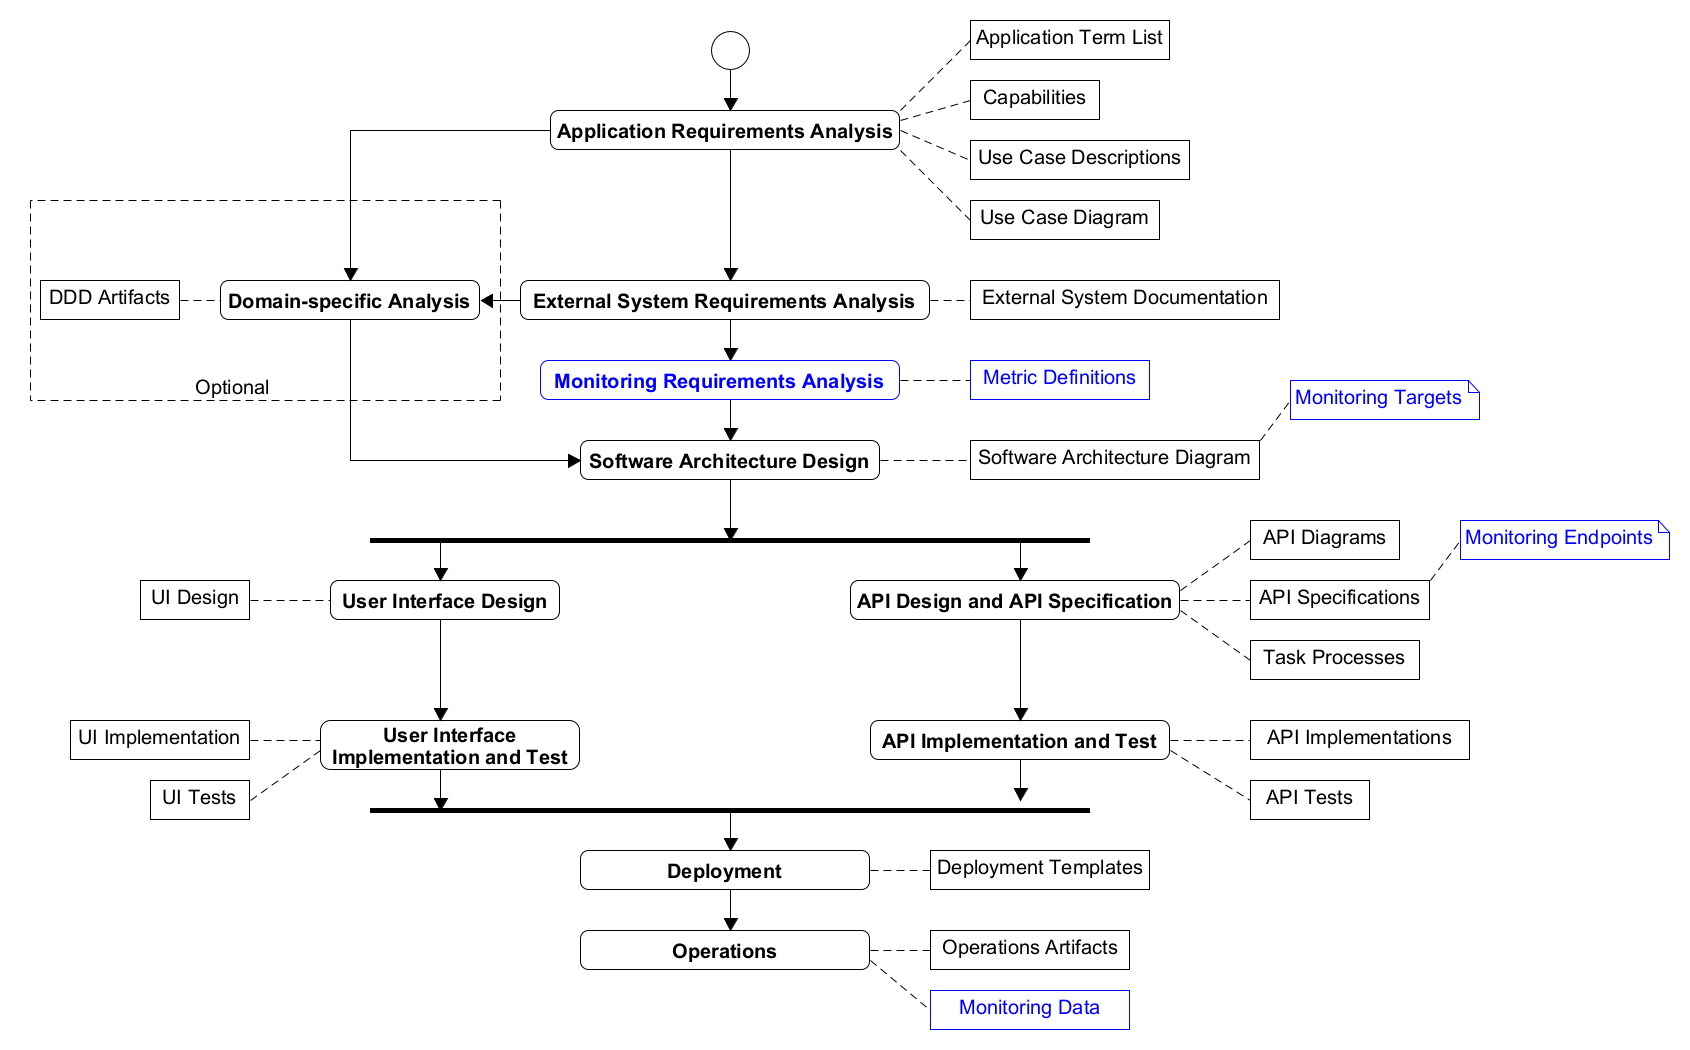
\includegraphics[width=\textwidth]{figures/4.3_ume_approach_extended.png}
	\caption{Extended Unified Microservice Engineering Approach}
	\label{fig:ume_approach_extended}
\end{figure}

In this section, the extension of the UME (Unified Microservice Engineering Approach) approach
by a monitoring concept is described. This represents the answer to the first research question
that was stated in Chapter \ref{cha:introduction}.

The extension of the UME approach with a monitoring concept is based on two assumptions.
The first assumption is that a viable monitoring system already exists.
This assumption is made because it simplifies the step API design and API specification in the extended UME approach
as can be seen later.
A monitoring system is deemed viable if it supports the aggregation of collected monitoring data
into new metrics. A viable monitoring system also needs to fulfill the second assumption that was made.
The second assumption is that the monitoring system works by pulling data from the application
as opposed to the data being sent to the monitoring system by the application.
By using this approach, the API of microservices that provide data to the monitoring system
can be explicitly extended by a monitoring endpoint. This aligns with
the API-oriented approach to designing microservices taken by the UME approach.

The extended UME approach can be seen in Figure \ref{fig:ume_approach_extended}.
The extension of the UME approach with a monitoring concept starts in the analysis phase
of the development process. After the application requirements analysis and external system requirements analysis,
a new analysis called monitoring requirements analysis is added.
The goal of this analysis step is to find metrics and define them.
Metrics can be found by analyzing the story on which an application is based.
In this way, the purpose of a metric should be directly related to an application's story.
After metrics have been identified, they need to be defined. This is done in the metric definitions artifact.
The metric definitions artifact is a list
that contains the definition of all metrics that should be monitored.
The definition of each metric consists of the metric's name, the purpose of the metric,
its type, a list of values necessary for calculating the metric, how the metric should
be represented visually and optionally different ranges of values of the metric with associated
state information. An example of a metric definition can be seen in Listing \ref{lis:metric_definition_example}.
The purpose of a metric should clarify the meaning of a metric and its usage.
An example of this can be seen in Listing \ref{lis:metric_definition_example} where the metric's
purpose is stated to be the identification of memory leaks within a service.
A metric can be categorized by the type of information that it provides and how it is calculated.
A metric is either a business metric or a technical metric and its method of calculation is either
elementary or through aggregation.
Business metrics capture the performance of business processes.
An example from BestRentalPoC is the number of issued digital driving licenses.
Technical metrics capture the state of the application as numerical values.
Examples of technical metrics are the four golden signals latency, traffic, errors, and saturation
as defined in Chapter \ref{cha:foundations}.
An elementary metric can be calculated from a single value captured from the application and does not
need any other information. Elementary metrics can be combined to form aggregated metrics
which are calculated by combining the values of different elementary metrics into a single value.
The list of values necessary for calculating the metric is used in a later step
of the extended UME approach to define monitoring targets in the software architecture of the application.
If the type of a metric is elementary then the list of values necessary for calculating the metric
must consist of exactly one entry. If the metric is aggregated then the list of values necessary for calculating
the metric should also state how the different values in the list are combined to form the aggregated metric.
The visual representation should describe how the metric can be presented in the chosen monitoring tool.
This description should be kept short. An example of such a description can be seen in Listing \ref{lis:metric_definition_example}.
Optionally, a metric's definition can contain value ranges that signal different states of a metric.
Taking the metric latency, possible value ranges would be: <1ms means latency is good, <10ms means high latency,
and >1s means critical latency. These states can then be used to, for example, trigger alerts or start
processes. For example, if the metric latency reaches the state of critical latency in a cloud application,
a process that might be started is to scale the application horizontally by adding more instances of services.

\begin{figure}[tb]
\begin{lstlisting}[caption = {Example of a Metric Definition}, label = {lis:metric_definition_example}, style = kit-cm, language=]
Name: Service A Memory Usage

Purpose:
Capture the amount of main memory being used by Service A
to identify memory leaks in the service's implementation.

Type: Elemental, Technical

Values:
- Service A: currently used main memory in bytes.

Visual Representation:
- Option A: Line Graph with time as the x-axis and the current metric value as the y-axis.
- Option B: Gauge with different colors for the different ranges of the metric.

Ranges:
- Ok: Value < 100 MB
- Warning: 100 MB < Value < 500 MB
- Critical: Value > 500 MB
\end{lstlisting}
\end{figure}

The next adaptation of the UME approach is in the software architecture design.
The main artifact of the software architecture design is the software architecture diagram.
The C\&M research group uses SPS (SystemPlusSoftware) diagrams for this purpose.
Based on the metrics defined during the monitoring requirements analysis,
microservices within the software architecture diagram are optionally marked as monitoring targets.
A monitoring target is a microservice that can provide values that are listed in a metric's definition.

The next change to the UME approach is the extension of the API specifications created during the
API design and API specification step. Microservices that have been marked as monitoring targets
during the software architecture design need to include monitoring endpoints in their API
through which the data that is being collected by the microservice can be collected by the monitoring system.
Because the assumption was made the monitoring system is chosen in advance,
the monitoring endpoint in the API specification can be designed to fit the monitoring system.

The last change to the UME approach is the addition of a new artifact to the operations step.
This new artifact is called monitoring data. In contrast to the other artifacts of the UME approach,
the artifact monitoring data is an abstract artifact. Monitoring data represents the insights
gained by analyzing the collected metrics. These insights can be gained from the visual representations
of the metrics in the monitoring system. Monitoring data can be used for the purposes stated
in the metric definitions to inform the decisions of future development work and business decisions.